% GENERATED by build_tex.py from paper2/draft/paper2_draft.md -- do not edit by hand
\begin{abstract}
Kolmogorov--Arnold networks (KANs) are promoted as interpretable because each edge carries a learned univariate function. We show that a widely used family of smoothness penalties leaves a blind spot that undermines this promise: second-difference and curvature penalties do not charge for affine components of an edge, and SiLU base weights are often unpenalised. When the inputs to a layer are correlated, affine components on different edges can cancel inside a unit, so training inflates the parameters along directions that neither the penalty nor the data can see; the loss has no reachable finite minimum and independent runs never agree. In a pre-registered synthetic study with a known teacher, correlated inputs gave 0 of 16 converged models (median squared-norm growth 32--66$\times$), including under a recently proposed curvature penalty that also penalises the SiLU weight, while a small penalty on the affine null space gave 16 of 16 certified minima and exact recovery of the teacher's internals. On real electrolyte-conductivity data the same mechanism explains why no model converged, and polishing beyond early stopping under a weak null-space penalty degraded held-out accuracy (RMSE 0.142 $\to$\allowbreak{} 1.03). Closing the blind spot restores certified minima but leaves several distinct minima, so convergence and identifiability are separate problems. We give practical recommendations for penalised KANs.

\end{abstract}

\section{Introduction}\label{sec:1}

KANs replace a network's fixed activations with learned univariate functions on every edge. Their appeal for science rests on reading those functions: an edge that looks like an exponential decay suggests a physical law. That reading presumes the edges are determined by the data. If different training runs produce different edges with equally good predictions, the edges describe the optimiser, not the system.

This paper identifies a concrete, common mechanism that breaks that presumption. It arises from the interaction of three ingredients that are each standard in practice:

\begin{enumerate}
  \item \textbf{A smoothness penalty with an affine null space.} Second-difference (P-spline) penalties and curvature penalties ignore straight-line components of an edge; SiLU base terms are frequently unpenalised.
  \item \textbf{Correlated inputs to a layer.} Physical descriptors often move together. Hidden units can also become correlated during training, exposing the next layer.
  \item \textbf{Training toward convergence.} Early stopping hides the problem; longer optimisation exposes it.
\end{enumerate}

Together they create directions along which edges grow into large, mutually cancelling affine shapes. The penalty does not see them, and on the training data their contributions cancel. The loss keeps decreasing slightly along these directions, so it has no reachable finite minimum. Seeds wander apart, no model certifies as converged, and on inputs off the training correlation pattern the cancellation fails.

\textbf{Contributions.}

\begin{itemize}
  \item We describe the mechanism and show that it applies to any layer whose inputs are correlated, including the output layer (Section 3).
  \item In a pre-registered synthetic study, we show causally that a recently proposed curvature penalty does not prevent the runaway on correlated inputs, while a small additional penalty on the affine null space prevents it and restores exact recovery of a known solution (Section 4).
  \item On real electrolyte-conductivity data, we trace a complete failure to converge to this mechanism and document its effect on extrapolation (Section 5).
  \item We show that closing the blind spot yields certified, isolated minima but not uniqueness, and that structured alternatives trade accuracy for stability (Section 6).
  \item We give recommendations for penalised KANs (Section 7).
\end{itemize}

All experiments were pre-registered: predictions, thresholds and interpretation rules were committed before the code that tested them. Of 65 predictions in the real-data case study, 11 held, 22 failed and 32 were inconclusive; we report them as recorded.

\section{Background and related work}\label{sec:2}

\textbf{KAN edges.} A KAN layer maps inputs to outputs by summing learned univariate functions, one per edge. In the original formulation \citep{liu2025kan} each edge is a SiLU base term plus a B-spline expansion. FastKAN \citep{li2024fastkan} approximates the B-splines with Gaussian radial basis functions on fixed centres, which is the edge type used in our experiments:

\begin{equation}
  \varphi(x) = \alpha\,\mathrm{SiLU}(x) + \sum_{k=1}^{K} c_k \exp\!\left(-\left(\frac{x-\mu_k}{h}\right)^{2}\right)
\end{equation}

\textbf{Smoothness penalties and their null spaces.} P-spline penalties charge squared second differences of the coefficients \citep{eilers1996psplines}. Constant and linear coefficient patterns cost nothing: the penalty's null space is affine. In generalised additive models this is well understood, and \citet{marra2011double} proposed an additional penalty on the null space (the "double penalty") for variable selection. Our fix is the same construction; what is new is its consequence inside a KAN, where edges are summed within units and passed through further layers.

\textbf{Curvature penalties for KANs.} \citet{bagrow2026curvature} proposed per-edge curvature penalties for compositional smoothness, combining the second-difference penalty with a term $K_{\mathrm{silu}}\,\alpha^{2}$ on the SiLU weight, and noted that the penalty has affine functions as its null space by design. That work evaluated on independent, uniformly sampled inputs. Second-derivative penalties on spline coefficients also appear in other KAN variants, typically on the spline part only, leaving the SiLU base term free (\citealp{cang2024kanwork}; see also the free-knots KAN of \citealp{zheng2025freeknots}). We show that the affine null space becomes a runaway direction when inputs are correlated, and that penalising the SiLU weight alone does not close it.

\textbf{Concurvity.} In additive models, correlated inputs let one input's shape function absorb another's, making shape functions non-identifiable; this is known as concurvity. \citet{siems2023concurvity} proposed a regulariser penalising correlations between transformed features. The cross-edge cancellation we describe is concurvity inside a KAN unit. In an additive model with a penalised null space it shifts shape between functions; combined with an unpenalised affine null space in a KAN, it becomes unbounded growth.

\textbf{Losses without a finite minimum.} When a loss attains its infimum only at infinity, gradient descent drives the parameter norm to diverge, slowly, and optimisation can continue while held-out performance worsens \citep{soudry2018implicit}. Our runaway is an instance of this behaviour created by a penalty's null space.

\textbf{Parameter-space symmetries.} Exact symmetries (unit permutations, sign flips) make parameters non-identifiable in tanh and RBF networks, and completeness results characterise them \citep{sussmann1992uniqueness,kurkova1994uniqueness}. KANs add continuous symmetries such as affine reparametrisations of hidden units. The runaway is not an exact symmetry: it is an approximate one, a nearly flat but tilted direction, which is what prevents convergence.

\section{Mechanism}\label{sec:3}

Consider a unit that sums edges from two inputs, $s = \varphi_1(x_1) + \varphi_2(x_2)$, each edge as in Section 2, trained with a second-difference penalty on its RBF coefficients.

\textbf{Step 1: a direction the penalty cannot see.} Add a linear pattern $t\,\ell$ to the RBF coefficients of edge 1 and subtract it from edge 2, with $\ell_k$ proportional to the centre index. Linear coefficient patterns have zero second difference, so the penalty is unchanged for every t (Figure~\ref{fig:mechanism}b). With Gaussian bumps on a regular grid, the pattern produces a nearly affine function: over the central 80\% of the input range it deviates from a straight line by at most 2\% of its range (Figure~\ref{fig:mechanism}a), and by up to 13\% near the grid edges. Edge 1 thus gains approximately $t\,a\,x_1$ and edge 2 loses $t\,a\,x_2$.

\textbf{Step 2: a direction the data cannot see.} The unit's pre-activation changes by approximately $t\,a\,(x_1 - x_2)$. If $x_{1}$ and $x_{2}$ are strongly correlated, $x_1 - x_2$ is small wherever the data lie, so predictions change little even for large t (Figure~\ref{fig:mechanism}c). The direction is nearly free in both the penalty and the data.


\begin{figure}[t]
  \centering
  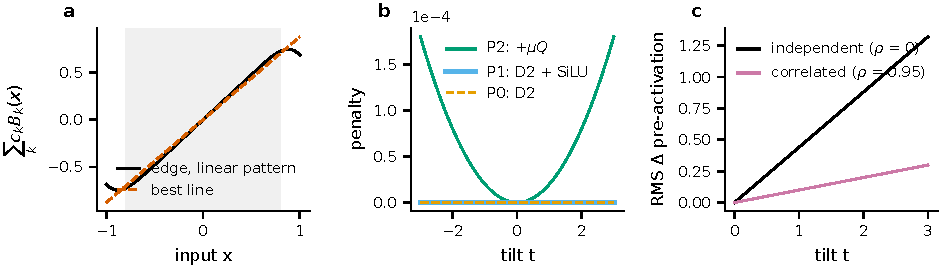
\includegraphics[width=\linewidth]{fig1_mechanism.pdf}
  % CAPTION-DRAFT: review (numbers from paper2/figures/fig1_mechanism.json)
  \caption{Mechanism (computed illustration) for the edge type of Section~\ref{sec:2} (8 Gaussian RBFs on $[-1, 1]$). \textbf{(a)} Edge function produced by a unit linear coefficient pattern and its best straight line; the shaded band is the central 80\% of the range, where the maximum deviation is 2.0\% of the function's range (12.9\% over the full range). \textbf{(b)} Penalty as a function of a tilt $t$ applied as $+t$ to edge 1 and $-t$ to edge 2: the second-difference penalty (P0) and P1 are exactly zero for every $t$; only P2's term $\mu Q$ grows ($\lambda = 0.001$, $\mu = 1e-05$). \textbf{(c)} RMS change in the unit's pre-activation per unit tilt: 0.0996 on correlated inputs ($\rho = 0.95$) against 0.4403 on independent inputs (4.42$\times$).}
  \label{fig:mechanism}
\end{figure}

\textbf{Step 3: no finite minimum.} "Nearly free" is not "free". Moving along it lets the model shed curvature into the free affine and SiLU components, so the loss decreases monotonically along the direction. Both terms contribute (post-hoc decomposition). In the synthetic runaway models the smoothness penalty fell to about a quarter of its early value and supplied a median 61\% of the decrease, while training error fell only 5\%. On real data, from early stopping to the capped state, the penalty fell 8--88$\times$ but supplied 17--36\% of the decrease, the data term the rest. In both, the growth went into whatever the penalty left free: the linear part of the RBF coefficients grew 34--40$\times$ in the synthetic runaway cells, and the SiLU weights 85$\times$ where they were unpenalised. In 12 of 20 synthetic runaway models, training error fell while test error rose. The infimum lies at infinity: gradients stay small but non-zero, the parameter norm grows without bound, and no minimum can be certified. Different seeds drift along different such directions.

\textbf{Step 4: any layer can be affected.} The argument needs only correlated inputs to a layer. Hidden units can become correlated during training, and then the output layer can host the same runaway even when the raw inputs are independent. Correlated hidden units appear necessary for this but not sufficient: they also occur in models that converge once the null space is penalised. Section 4 shows both forms.

\textbf{Consequences.}

\begin{itemize}
  \item \textbf{Non-identifiability:} edges differ across seeds by large affine components that leave predictions almost unchanged.
  \item \textbf{Non-convergence:} second-order optimisers stall; certification criteria fail.
  \item \textbf{Extrapolation risk:} off the training correlation pattern, $x_1 - x_2$ is no longer small, and the inflated components stop cancelling.
\end{itemize}

\textbf{The fix.} Penalise the null space directly. For each edge, let $P_{\mathrm{null}}$ project its RBF coefficients onto constant-plus-linear patterns in the centre index, and add

\begin{equation}
  Q = \sum_{e} \lVert P_{\mathrm{null}}\, c_e \rVert^{2}
\end{equation}

with a small weight $\mu$, in addition to a penalty on the SiLU weight. This makes every affine component cost something, which turns the infinite descent into a finite minimum.

\section{Controlled study}\label{sec:4}

\textbf{Design.} A teacher KAN [4, 3, 1] with smooth, hand-specified edges (fitted by smoothness-penalised least squares) generates targets with Gaussian noise of 5\% of the output spread; n = 2000 training rows. Inputs are $\mathcal{N}(0, 1)/3$, clipped to the grid, either independent or correlated in pairs ($\rho$ = 0.95 for $x_1/x_2$ and $x_3/x_4$). Students share the teacher's architecture and are trained under three penalty levels:

\begin{itemize}
  \item \textbf{P0:} second-difference penalty on RBF coefficients ($\lambda$ = $10^{-3}$).
  \item \textbf{P1:} P0 plus $K_{\mathrm{silu}}\,\alpha^{2}$ on each SiLU weight (Bagrow-style curvature penalty, $K_{\mathrm{silu}}$ = 0.443).
  \item \textbf{P2:} P1 plus $\mu Q$, the affine null-space penalty.
\end{itemize}

Each of the 6 cells has 8 seeds. Each student is trained with AdamW and early stopping, then polished with an exact-Hessian trust-region method and certified by a second-order criterion (gradient, curvature and Newton decrement). $\mu$ was calibrated before the experiment by a pre-registered rule: $10^{-6}$ failed the pilot (5.0$\times$ growth) and $10^{-5}$ passed (1.32$\times$) and was frozen.

\textbf{The teacher itself runs away.} Polished under P0 and P1 on correlated inputs, the teacher's parameters grew 85$\times$ and 1069$\times$ without certifying, while its predictions stayed within half a noise standard deviation of the original. The runaway changes the parameters, not the function.

\begin{table}[t]
  \centering
  % CAPTION-DRAFT: review
  \caption{Synthetic $2\times3$ study, per cell.}
  \label{tab:synthetic}
  \small
  \begin{tabular}{lp{0.2\linewidth}p{0.2\linewidth}p{0.2\linewidth}p{0.2\linewidth}p{0.2\linewidth}p{0.2\linewidth}p{0.2\linewidth}p{0.2\linewidth}p{0.2\linewidth}p{0.2\linewidth}p{0.2\linewidth}p{0.2\linewidth}p{0.2\linewidth}p{0.2\linewidth}p{0.2\linewidth}p{0.2\linewidth}p{0.2\linewidth}p{0.2\linewidth}p{0.2\linewidth}p{0.2\linewidth}p{0.2\linewidth}p{0.2\linewidth}p{0.2\linewidth}p{0.2\linewidth}p{0.2\linewidth}p{0.2\linewidth}p{0.2\linewidth}p{0.2\linewidth}p{0.2\linewidth}p{0.2\linewidth}p{0.2\linewidth}p{0.2\linewidth}p{0.2\linewidth}p{0.2\linewidth}p{0.2\linewidth}p{0.2\linewidth}p{0.2\linewidth}p{0.2\linewidth}p{0.2\linewidth}p{0.2\linewidth}p{0.2\linewidth}p{0.2\linewidth}p{0.2\linewidth}p{0.2\linewidth}p{0.2\linewidth}p{0.2\linewidth}p{0.2\linewidth}p{0.2\linewidth}p{0.2\linewidth}p{0.2\linewidth}p{0.2\linewidth}p{0.2\linewidth}p{0.2\linewidth}p{0.2\linewidth}p{0.2\linewidth}p{0.2\linewidth}p{0.2\linewidth}p{0.2\linewidth}p{0.2\linewidth}}
  \toprule
  Cell & Norm growth & Certified & Unit match to reference \\
  \midrule
  Independent, P0 & 12.5$\times$ & 6/8 & 1.000 \\
  Independent, P1 & 7.9$\times$ & 6/8 & 1.000 \\
  Independent, P2 & 1.09$\times$ & 8/8 & 1.000 \\
  Correlated, P0 & 65.7$\times$ & 0/8 & 0.774 \\
  Correlated, P1 & 32.1$\times$ & 0/8 & 0.883 \\
  Correlated, P2 & 1.00$\times$ & 8/8 & 1.000 \\
  \bottomrule
  \end{tabular}
\end{table}

Medians over 8 seeds; growth is the squared parameter norm, polished over early-stopped.

\textbf{Results.}

\begin{itemize}
  \item \textbf{The published-style penalty does not prevent the runaway.} Penalising the SiLU weight (P1) halved the growth on correlated inputs but left 0 of 8 models certified (Figure~\ref{fig:synthetic}).
  \item \textbf{Closing the null space prevents it everywhere.} P2 gave 16 of 16 certified models with no growth, in both input conditions.
  \item \textbf{Without the runaway, the internals are recoverable.} Every cell without a runaway matched the reference's units and edges exactly (1.000), with seed-to-seed differences around $10^{-4}$.
  \item \textbf{Independent inputs are not fully safe.} Under P0 and P1, most independent seeds grew substantially (8--12$\times$) but settled at certified minima; 4 of 16 (seeds 0 and 4 in each cell) never certified.
\end{itemize}


\begin{figure}[t]
  \centering
  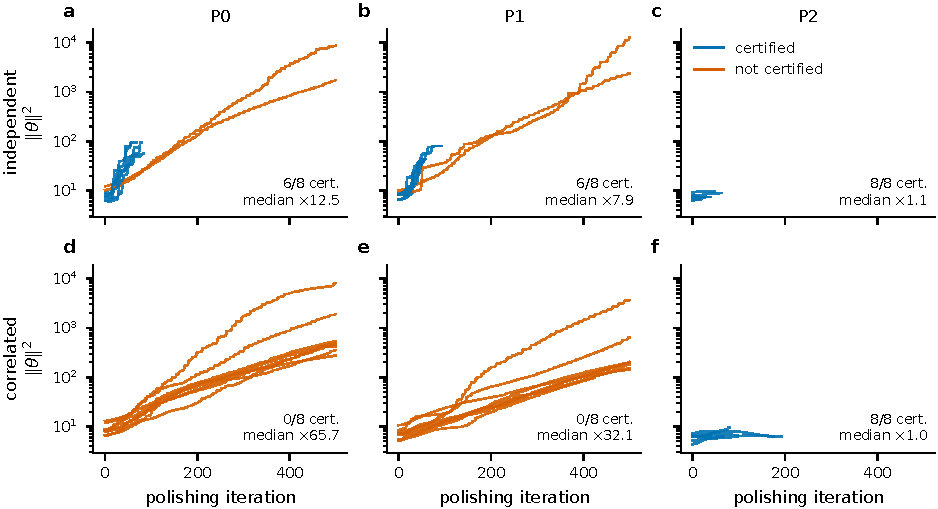
\includegraphics[width=\linewidth]{fig2_synthetic.pdf}
  % CAPTION-DRAFT: review (numbers from paper2/figures/fig2_synthetic.json)
  \caption{Synthetic $2\times3$ study: $\|\theta\|^2$ over trust-exact polishing iterations (log scale), one line per seed, coloured certified (blue) or not certified (vermillion). Rows: independent and correlated inputs; columns: P0, P1, P2. Per panel, certified seeds and median growth (polished over early-stopped): independent P0: 6/8 certified, $\times$12.5; independent P1: 6/8 certified, $\times$7.9; independent P2: 8/8 certified, $\times$1.1; correlated P0: 0/8 certified, $\times$65.7; correlated P1: 0/8 certified, $\times$32.1; correlated P2: 8/8 certified, $\times$1.0.}
  \label{fig:synthetic}
\end{figure}

\textbf{Where the runaway lives.} A post-hoc anatomy of the parameter change shows that in the correlated cells almost all growth sits in the output layer: the layer-1 share of the change was 0.110 (P0) and 0.024 (P1) (Figure~\ref{fig:where}a). It went into the affine part of the output edges' RBF coefficients and, under P0, into their SiLU weights. Cancellation across the edges entering the output rose from about 1.9 to 3.1--3.2, and no hidden unit saturated. The two uncertified independent-P0 seeds put 99.4\% of their change into the output layer. This is Step 4 of Section 3. Among independent-input models, those that ran away were exactly those whose hidden units had become correlated (largest pairwise correlation 0.70, against 0.05 for certified models; Figure~\ref{fig:where}b), while certified P2 models kept correlations up to 0.88 without running away (post-hoc).


\begin{figure}[t]
  \centering
  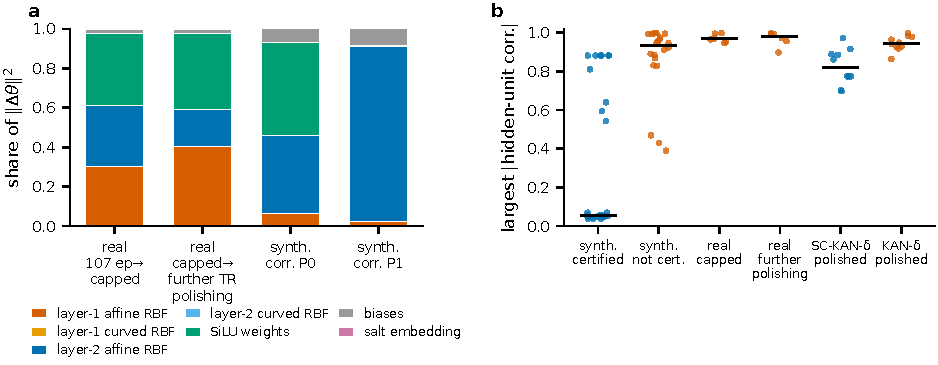
\includegraphics[width=\linewidth]{fig4_where.pdf}
  % CAPTION-DRAFT: review (numbers from paper2/figures/fig4_where.json)
  \caption{Where the runaway lives. \textbf{(a)} Mean share of $\|\Delta\theta\|^2$ by parameter block. Real data, 107 epochs$\to$capped: layer-1 affine RBF 0.30, layer-2 affine RBF 0.31, SiLU weights 0.37; capped$\to$Part~A: 0.40, 0.19, 0.38; synthetic correlated P0: layer-2 affine RBF 0.39, SiLU weights 0.47; correlated P1: layer-2 affine RBF 0.89. The real-data split was evaluated post hoc from archived weights (Appendix~\ref{app:repro}). \textbf{(b)} Largest absolute correlation between hidden-unit activations on the training rows, median: synth. certified 0.054 ($n=28$); synth. not cert. 0.935 ($n=20$); real capped 0.968 ($n=6$); real Part A 0.983 ($n=6$); SC-KAN-$\delta$ polished 0.818 ($n=10$); KAN-$\delta$ polished 0.946 ($n=10$). Blue: certified; vermillion: not certified or runaway.}
  \label{fig:where}
\end{figure}

\textbf{Verdicts.} Of six pre-registered predictions, one held (the certification pattern, X2) and five failed. The failures refine rather than contradict the mechanism. Independent cells exceeded the growth threshold, mostly through finite growth. Cancellation and extrapolation effects were weaker than predicted. Recoverability failed only because the runaway cells were more recoverable than predicted, not less. In this synthetic setting, polishing did not degrade extrapolation: most of the off-pattern error in correlated cells was present at early stopping.

\section{Real-data case study: electrolyte conductivity}\label{sec:5}

\textbf{Task and model.} The CALiSol-23 challenge \citep{deblasio2024calisol} asks for the log conductivity of lithium-ion electrolytes; every test sample contains diethyl carbonate (DEC), which never appears in training. KAN-delta anchors each prediction on the measured conductivity of pure propylene carbonate (PC) and learns only the correction, $\log k = \log k_{\mathrm{PC}} + x_{\mathrm{co}}\, h(z)$, where h is a FastKAN-style network of shape [10, 6, 1]. Its inputs are physical descriptors of the solvents (dielectric constant, log viscosity, molar mass), temperature, molality and a salt embedding. A second-difference penalty acts on the RBF coefficients, and the SiLU weights are unpenalised. Early-stopped after 107 AdamW epochs, it reached RMSE 0.142 on a held-out co-solvent.

\textbf{The inputs are correlated and few-valued.} The three co-solvent descriptors take only 30 distinct combinations in training, and dielectric constant and log viscosity correlate at r = 0.966.

\textbf{Nothing ever converged.}

\begin{itemize}
  \item Of 190 pairs of polished independent seeds, none computed the same function.
  \item After 20,000 float64 L-BFGS iterations, 0 of 26 models converged; exact-Hessian trust-region methods also failed on every seed.
  \item Students trained on a frozen teacher matched its predictions (correlation 0.9988) but not its hidden units (0.66).
\end{itemize}

\textbf{The anatomy matches Section 3.}

\begin{itemize}
  \item From early stopping to the capped state, the squared parameter norm grew 150--1550$\times$ while the smoothness penalty fell 8--88$\times$.
  \item At least 99.9\% of the coefficient change during exact-Newton polishing lay in the penalty's affine null space, in 9 of 9 models.
  \item Cancellation within an edge (SiLU against RBF) stayed small, 1.13--1.33. Cancellation across the edges entering a unit rose from 1.7--2.9 to 4--10, consistent with the correlated descriptors.
  \item The runaway spread across both layers: 30--40\% of the parameter change went into layer-1 affine RBF coefficients, 37--38\% into SiLU weights and 19--31\% into layer-2 affine coefficients (post-hoc), and 12--39\% of hidden units saturated. In the synthetic runaway the output layer dominated.
\end{itemize}

\textbf{Extrapolation suffered.} Polishing beyond early stopping, under a weak null-space penalty, raised the held-out RMSE from 0.142 to 1.03. The cancelling components appear to stop cancelling on the unseen co-solvent, whose descriptors sit off the training correlation pattern. This degradation was much stronger than in the synthetic study, where correlation itself caused most of the off-pattern error; the real model was larger, its norms grew further, and the test solvent lay at the edge of the descriptor range.

\section{Closing the blind spot, and what remains}\label{sec:6}

\textbf{Dose-response on real data.} Adding $\mu Q$ (with the SiLU weights included in Q) and polishing from the early-stopped weights:

\begin{table}[t]
  \centering
  % CAPTION-DRAFT: review
  \caption{Dose-response in $\mu$ on real data (seeds).}
  \label{tab:dose}
  \small
  \begin{tabular}{l l p{0.18\linewidth} l p{0.16\linewidth}}
  \toprule
  $\mu$ & Seeds at a numerical minimum & Negative curvature (seeds) & Norm growth (seeds) & Training fit vs runaway \\
  \midrule
  $10^{-6}$ & 0 of 6 & up to 9 eigenvalues & 21--31$\times$ & about equal \\
  $10^{-5}$ & 4 of 6 & up to 4 eigenvalues & 9--43$\times$ & 12--22\% worse \\
  $10^{-4}$ & 6 of 6 & none & 1.6--16$\times$ & 15--39\% worse \\
  \bottomrule
  \end{tabular}
\end{table}

Under a second-order certificate, all six seeds at $\mu$ = $10^{-4}$ were certified (Figure~\ref{fig:dose}). (The originally pre-registered criterion, which required 10 stationary iterations, proved unreachable because the optimiser stops a few iterations after reaching a minimum; the certificate was defined afterwards and is reported alongside the original verdict.) Saturation fell to at most 0.5\% and cross-edge cancellation to 2.2--2.9.


\begin{figure}[t]
  \centering
  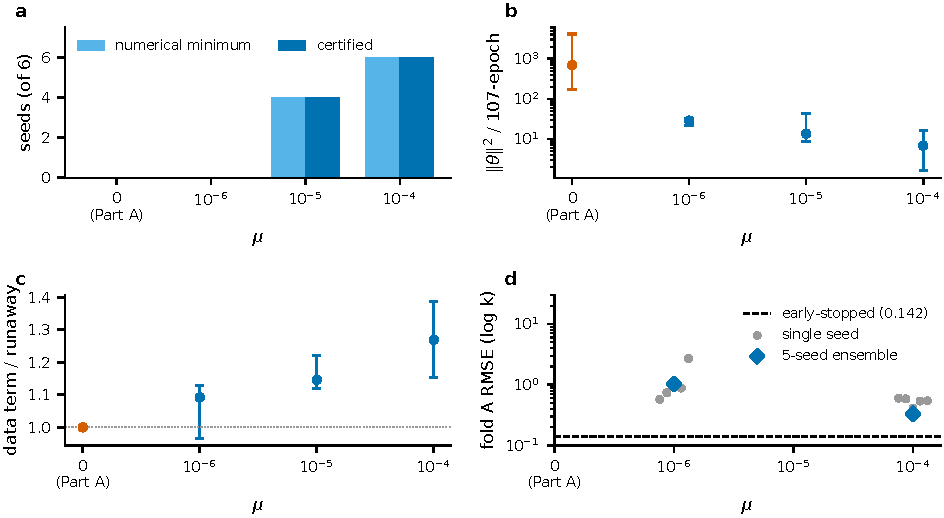
\includegraphics[width=\linewidth]{fig3_dose_response.pdf}
  % CAPTION-DRAFT: review (numbers from paper2/figures/fig3_dose_response.json)
  \caption{Real-data dose-response in the null-space weight $\mu$ (6 KAN-delta seeds; $\mu = 0$ is the runaway reference, stage-2 Part~A). \textbf{(a)} Seeds at a numerical minimum / certified: 0: 0/0; 1e-06: 0/0; 1e-05: 4/4; 0.0001: 6/6. \textbf{(b)} $\|\theta\|^2$ relative to the 107-epoch state, median (range): 0: 690.0 (170.0--4145.5); 1e-06: 28.8 (21.2--31.5); 1e-05: 13.6 (8.6--43.1); 0.0001: 6.8 (1.6--16.0). \textbf{(c)} Training data term relative to the runaway, median: 1e-06: 1.092; 1e-05: 1.146; 0.0001: 1.269. \textbf{(d)} Fold A RMSE: early-stopped 0.142 (dashed line); polished 5-seed ensemble 1.026 at $\mu = 10^{-6}$ and 0.334 at $\mu = 10^{-4}$; grey points are single seeds.}
  \label{fig:dose}
\end{figure}

\textbf{A known solution becomes recoverable.} Under the regularised loss, the original teacher is no longer a minimum. Optimising it under the same loss gives a "regularised teacher" computing nearly the same function (correlation 0.9992). Students match its units at 0.87--0.90 and its edges at 0.97--0.98, against 0.68--0.72 and 0.84--0.91 for the original teacher. This comparison was defined after the results and is exploratory.

\textbf{The penalty acts partly as gauge fixing.} At the certified minima, the layer-2 constant shift, an essentially exact symmetry, owes 96\% of its curvature to $\mu Q$: the regulariser selects one representative. The layer-1 constant shift (46\%) and unit rescaling (24\%) are only approximate symmetries in this architecture, because Gaussian bumps cannot represent constants exactly and tanh breaks rescaling.

\textbf{Convergence is not uniqueness.} Independent seeds at certified minima still disagreed: their median prediction difference fell by only 26\% (Figure~\ref{fig:uniqueness}b). With the runaway removed, the loss has several distinct isolated minima.


\begin{figure}[t]
  \centering
  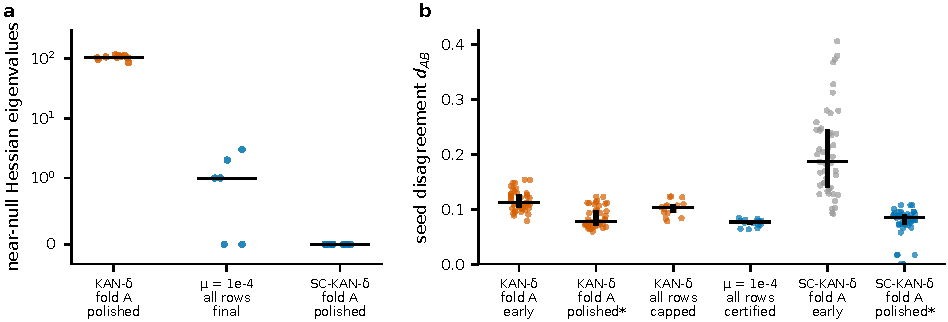
\includegraphics[width=\linewidth]{fig5_uniqueness.pdf}
  % CAPTION-DRAFT: review (numbers from paper2/figures/fig5_uniqueness.json)
  \caption{Convergence is not uniqueness. \textbf{(a)} Near-null Hessian eigenvalues ($|\lambda| < 10^{-8}\lambda_{\max}$) at the end of polishing: KAN-delta baseline on fold A, median 106 (range 86--116); null-space penalty $\mu = 10^{-4}$ on all rows, median 1 (range 0--3); SC-KAN-delta on fold A, 0--0. \textbf{The baseline counts are taken at non-stationary points}: none of the 10 baseline models was certified, and all stopped at the 500-iteration cap. \textbf{(b)} Seed disagreement $d_{AB}$ (median, interquartile range): KAN-$\delta$ fold A early 0.112; KAN-$\delta$ fold A polished$^*$ 0.077; KAN-$\delta$ all rows capped 0.104; $\mu$ = 1e-4 all rows certified 0.077; SC-KAN-$\delta$ fold A early 0.187; SC-KAN-$\delta$ fold A polished$^*$ 0.085. Groups marked $^*$ (polished fold A) are not in any committed result: they were evaluated post hoc from the archived polished weights (SHA-verified; predictions on the 1434 fold A training rows), without any re-optimisation.}
  \label{fig:uniqueness}
\end{figure}

\textbf{Extrapolation.} On the held-out co-solvent, RMSE was 0.142 for the early-stopped model, 1.026 after polishing at $\mu$ = $10^{-6}$ and 0.33 at $\mu$ = $10^{-4}$. Bounding the runaway recovers most of the damage, but early stopping remains the most accurate choice.

\textbf{Structured alternatives.} We tested two architectures designed to remove runaway routes by construction, against the early-stopped baseline, with leave-one-co-solvent-out (LOCO) validation:

\begin{table}[t]
  \centering
  % CAPTION-DRAFT: review
  \caption{Structured alternatives against the early-stopped baseline.}
  \label{tab:alternatives}
  \small
  \begin{tabular}{l p{0.24\linewidth} l l p{0.16\linewidth}}
  \toprule
  Model & Idea & LOCO RMSE & Converged & Seed agreement \\
  \midrule
  Baseline KAN-delta & As above & 0.255 & 0/10 & 0.112 \\
  Shared-curve KAN & One curve per input, mixed by penalised weights & 0.292 & 10/10 & 0.187 early; 0.085 polished \\
  Two-anchor excess model & Pure-solvent offset plus $x(1 - x)$ mixing term & 0.283 & not tested & not tested \\
  \bottomrule
  \end{tabular}
\end{table}

Seed agreement is the median prediction difference between seeds (lower is better). The shared-curve model converged every time, ending with no near-flat directions where the baseline had a median of 106 (range 86--116, at non-stationary points; Figure~\ref{fig:uniqueness}a), and it was less accurate. At the early-stopped state its seeds agreed less than the baseline's (the pre-registered comparison); after polishing to certified minima their median disagreement fell to 0.085, with some seed pairs reaching the same minimum (post-hoc). The excess model's "pure co-solvent offset" tracked viscosity rather than dielectric constant (rank correlation $-$0.85, post hoc), reflecting that no training row contains a pure co-solvent.

\section{Recommendations for practitioners}\label{sec:7}

\begin{enumerate}
  \item \textbf{Penalise the affine null space and the SiLU weights.} If a KAN uses a second-difference or curvature penalty, add a small penalty on the constant-plus-linear component of each edge's coefficients and on each SiLU weight, in every layer. Calibrate its weight so it barely moves a known smooth solution.
  \item \textbf{Check input correlations, including between hidden units.} Strongly correlated or few-valued inputs make the first layer vulnerable; any hidden layer can expose the next one.
  \item \textbf{Monitor parameter norms, not only the loss.} Steady norm growth with a slowly falling loss and stubborn gradients is the signature of the runaway. Certify convergence with a second-order criterion rather than assuming it.
  \item \textbf{Do not read edges from unconverged models.} Compare edges across seeds only after removing exact gauge freedoms, and only for models that reached certified minima.
  \item \textbf{Treat seed disagreement as information.} Even at certified minima, distinct solutions can remain. Disagreement then signals that the data do not determine the function, not merely that training was unfinished.
  \item \textbf{Validate on genuinely new conditions.} A held-out fold from the training distribution can understate extrapolation error severalfold; leave-one-group-out validation is closer to the use case.
  \item \textbf{Keep early stopping as a baseline.} In our real-data case it gave the best held-out accuracy of every variant tested.
\end{enumerate}

\section{Limitations and research process}\label{sec:8}

\textbf{Scope.}

\begin{itemize}
  \item One real dataset and one synthetic teacher; small networks ([4, 3, 1] and [10, 6, 1]).
  \item One edge type: Gaussian RBFs on fixed centres with a SiLU base. The argument applies to B-spline KANs with second-difference or curvature penalties, but we did not test them directly.
  \item Our P1 keeps the second-difference penalty on RBF coefficients and adds Bagrow's SiLU term; it is Bagrow-style, not a replication of his RBF curvature form.
  \item The null-space weight used in the shared-curve model was carried over from the synthetic calibration, not re-calibrated.
\end{itemize}

\textbf{Post-hoc elements.} The second-order certificate, the regularised-teacher comparison, the gauge-curvature analysis and both anatomy studies were defined after seeing results. We report them as exploratory and never in place of pre-registered verdicts.

\textbf{Extrapolation.} The strong degradation from polishing appeared on real data but not in the synthetic study, so we do not claim it as a general law.

\textbf{Process.} Each study committed its predictions, thresholds and interpretation rules before its code existed; any later change was dated and recorded as an amendment, and every verdict is linked to the commit that produced it. Several predictions failed or proved untestable as specified; following them up, rather than reinterpreting them, is what led to the mechanism reported here. Experiments were run with an AI coding agent working under this protocol, with a rule that committed files take precedence over any number stated in a prompt.
